\subsection{\Acrshort{pwm}-Erzeugung}

Um die Geschiwindigkeit eines Lüfters zu regulieren, wird dieser mit einem \gls{pwm} Signal gesteuert.
Die Pulsweite ist proportional zur resultierenden Zielgeschiwindigkeit.
Der \gls{rpi} hat interne Hardware um \gls{pwm} Signale zu generieren.
Diese sind jedoch nicht trivial aus dem Kernelspace erreichbar.

Als Ersatzlösung wird externe Hardware genutzt.
Ein \texttt{555} Timer erstellt ein rechteckiges Wechselsignal.
Die Pulsweite wird durch ein \texttt{MCP41XXX} digitales Potentiometer über \gls{spi} eingestellt.
Folglich ist die Lüftergeschwindigkeit proportional zur Pulsweite und proportional zum eingestellten Wiederstand.

\subsubsection{SPI Bus}

SPI ist ein synchroner, serieller Datenbus mit der Funktionsweise nach dem Master-Slave-Prinzip.
Die vier wichtigsten Leitungen sind \gls{sclk}, \gls{mosi}, \gls{miso} und \gls{ss}.
Die \gls{sclk} gibt einen Takt mit einer möglichen Frequenz bis $\si{\mHz}$ aus, welche zur Synchronisation vom Controller benötigt wird. Dieses Signale wird vom Master ausgegeben.
Mit \gls{ss} wird der jeweilige Slave ausgewählt, indem das Signal auf logisch 0 gesetzt wird.
Daten werden mit der \gls{mosi} Leitung vom Master zum Slave und mit der \gls{miso} Leitung vom Slave zum Master gesendet. \\
In \autoref{fig:spi-transaction} ist die Funktion von \gls{spi} dargestellt.
Wenn der Slave ausgewählt wurde, toggelt der \gls{ss} von logisch 1 auf logisch 0.
Mit jedem \gls{sclk} Takt wird ein Bit von Master auf Slave übertragen.
Nach Beenden der Übertragung toggelt der \gls{ss} wieder auf logisch 1.
Dies funktioniert mit der \gls{miso} Leitung vice versa.

\begin{figure}
    \begin{center}
    \begin{tikztimingtable}[%
        timing/dslope=0.2,
        timing/.style={x=1.6ex,y=2ex},
        x=1ex,
        timing/rowdist=4ex,
        timing/c/rising arrows,
        timing/name/.style={font=\sffamily\scriptsize},
    ]
    \busref{CS} & HHL;16{L};LHH\\
    \busref{SCK} & UULL;16{C};UU\\
    \busref{SO} & UUU;2D{D7};2D{D6};2D{D5};2D{D4};2D{D3};2D{D2};2D{D1};2D{D0};UUU\\
    %
    \extracode
    \begin{pgfonlayer}{background}
        \begin{scope}[semitransparent ,semithick]
            \vertlines[darkgray,dotted]{0,3.2 ,...,36.0}%
        \end{scope}
        \end{pgfonlayer}
    \end{tikztimingtable}
    \end{center}
    \caption[Eine \gls{spi} Datenübertragung.]{Eine \gls{spi} Datenübertragung von 8 Bits}
    \label{fig:spi-transaction}
\end{figure}

\subsubsection{MCP41XXX Digitales Potentiometer}

Die Schaltung des digitalen Potentiometers wird direkt an den \gls{rpi} angeschlossen.
Die Pins werden wie in \autoref{tab:spi} verbunden.
Der \texttt{MCP41XXX} hat zwei interne digital steuerbare Potentiometer.
Um deren Wiederstandswert einzustellen müssen zwei Bytes über \gls{spi} gesendet werden.
Das erste Byte stellt das Command-Byte dar.
Das zweite Byte die tatsächlichen Daten.
Die in \autoref{fig:spi-mcp-transaction} aufgeführten Bits in der Datenübertragung setzen sich aus dem Command-Byte und aus einem folgenden Datenbyte zusammen.
Die Bedeutung des Command-Byte wird in \autoref{tab:command-bits} erklärt.
Das Datenbyte setzt sich aus den folgenden 8 Bits (D7, \ldots, D0) zusammen.
Der resultierende Wiederstand zwischen Anschluss A und W kann mit der \autoref{eq:resistance1} berechnet werden.
Der Wiederstand zwischen B und W ist mit \autoref{eq:resistance2} zu berechenen.

\begin{table}[h]
    \centering
    \begin{tabular}{|r||l|l|l|l|l|}
        \hline
        \textbf{Funktion} & \textbf{\acrshort{mosi}} & \textbf{\acrshort{miso}} & \textbf{\acrshort{vcc}} & \textbf{\acrshort{sclk}} & \textbf{\acrshort{ss}} \\
        \hline
        \hline
        \gls{rpi} Pin Name & GPIO10 & GPIO9 & 5V Power & GPIO11 & GPIO8 \\
        \hline
        \gls{rpi} Pin Nummer & Pin19 & Pin21 & Pin2 & Pin23 & Pin24 \\
        \hline
    \end{tabular}
    \caption{\gls{spi} Pinout Tabelle}
    \label{tab:spi}
\end{table}

\begin{figure}[h]
    \begin{center}
    \begin{tikztimingtable}[%
        timing/dslope=0.2,
        timing/.style={x=1.6ex,y=2ex},
        x=1ex,
        timing/rowdist=4ex,
        timing/c/rising arrows,
        timing/name/.style={font=\sffamily\scriptsize},
    ]
    \busref{CS} & HHL;32{L};LHH\\
    \busref{SCK} & UULL;32{C};UU\\
    \busref{SO} & UUU;2D{X};2D{X};2D{C1};2D{C0};2D{X};2D{X};2D{P1};2D{P0};2D{D7};2D{D6};2D{D5};2D{D4};2D{D3};2D{D2};2D{D1};2D{D0};UUU\\
    %
    \extracode
    \begin{pgfonlayer}{background}
        \begin{scope}[semitransparent ,semithick]
            \vertlines[darkgray,dotted]{0,3.2 ,...,36.0}%
        \end{scope}
        \end{pgfonlayer}
    \end{tikztimingtable}
    \end{center}
    \caption[Eine \gls{spi} Datenübertragung für ein MCP41XXX Potentiometer]{Eine \gls{spi} Datenübertragung für ein MCP41XXX Potentiometer}
    \label{fig:spi-mcp-transaction}
\end{figure}

\begin{table}[H]
    \centering
    \begin{subtable}[t]{5cm}
        \centering
        \begin{tabular}{|l|l|l|}
            \hline
            \textbf{C1} & \textbf{C0} & \textbf{Kommando} \\
            \hline
            \hline
            0 & 0 & Kein Kommando \\
            \hline
            0 & 1 & Daten Schreiben \\
            \hline
            1 & 0 & Ausschalten \\
            \hline
            1 & 1 & Kein Kommando \\
            \hline
        \end{tabular}
        \caption{Kommando Bits}\label{command:1a}
    \end{subtable}
    \quad
    \begin{subtable}[t]{5cm}
        \centering
        \begin{tabular}{|l|l|l|}
            \hline
            \textbf{P1} & \textbf{P0} & \textbf{Kommando} \\
            \hline
            \hline
            0 & 0 & Kein Potentiometer \\
            \hline
            0 & 1 & Nur Potentiometer 0 \\
            \hline
            1 & 0 & Nur Potentiometer 1 \\
            \hline
            1 & 1 & Beide Potentiometer \\
            \hline
        \end{tabular}
        \caption{Potentiometer bits}\label{command:1b}
    \end{subtable}
    \caption{MCP41XXX Command-Byte Bits}
    \label{tab:command-bits}
\end{table}

\clearpage

\begin{samepage}
\begin{equation}
    R_{\text{\text{WA}}}(D_{\text{n}}) = \frac{(R_{\text{AB}}) (256 - D_{\text{n}})}{256} + R_{\text{W}}
    \label{eq:resistance1}
\end{equation}
\begin{equation}
    R_{\text{WB}}(D_{\text{n}}) = \frac{(R_{\text{AB}}) (D_{\text{n}})}{256} + R_{\text{W}}
    \label{eq:resistance2}
\end{equation}
wobei
\begin{align*}
    R_{\text{AB}} &: \text{Wiederstand zwischen Anschluss A und B, hier: } 10\si{k\ohm} \\
    R_{\text{W}} &: \text{Wiper Wiederstand, nominal: } 52\si{\ohm}  \\
    D_{\text{n}} &: \text{Dezimalwert des Wiperregisters: } 0_{10} \leq D_{\text{n}} \leq 255_{10}
\end{align*}
\end{samepage}

\subsubsection{555 Timer}

Der Timer ist in einer astabilen Konfiguration verbunden.
Der Timer erwartet lediglich eine Positive Spannung über $U+$ zu $U-$ von $3.3\si{\volt}$.
Ein rechteckiges Ausgangssignal mit einstellbarer Pulsweite wird an Pin 7, \texttt{DIS}, oder auch and Pin 3, \texttt{OUT}, gegben.
\texttt{DIS} ist Open-Drain womit der High-Pegel zu einer belibigen Spannung eingestellt werden kann.
Eine analytische Bestimmung von $U_C(t)$ oder $I(t)$ kann aufgrund der nicht linearen Übertragungsfunktion der Diode nicht bestimmt werden \autocite{rdc}.
Folglich ist eine berechnung von $f$ nicht möglich\footnote{Eine grobe Annäherung durch die Annahme, dass $U_{fd}$ der Dioden konstant und unabhängig von $I$ ist, ist möglich, jedoch sind die resultate daraus sehr ungenau und nahezu unbrauchbar.}.
Die Frequenz kann lediglich empirisch durch Messung oder Simulation ermittelt werden.

\begin{figure}[p]
    \centering
    \begin{tikzpicture}[
        %Global Config
        font=\small
    ]
    %You can create an smart objet like Henry Menke in this post http://www.texample.net/tikz/examples/4-bit-counter/
    % Variables: 1: Position 2: ID.
    \def\TIMER555(#1)#2{%
    \begin{scope}[shift={(#1)}]
        \draw[fill=blue!10] (-1.5,-2) rectangle (1.5,2); % The body of IC
        % Label and component identifier.
        % \draw[blue] (2,2.5) node []{\large \bf U - #2}; % IC LABEL
        \draw[blue] (0,0.5) node [align=center]{\large NE-555\\TIMER}; % IC LABEL
        % Draw the pins
        % Some that you have to learn about label nodes, draw lines, and name coordinates in Tikz
        \draw (0.9,-2) node [above]{GND} -- +(0,-0.5) node [anchor=-45]{1} coordinate (#2 GND); % Pin 1 GND
        \draw (-1.5,-1.5) node [right]{TRG} -- +(-0.5,0) node [anchor=-135]{2} coordinate (#2 TRG); % Pin 2 TRG
        \draw (1.5,0) node [left]{OUT} -- +(0.5,0) node [anchor=-45]{3} coordinate (#2 OUT); % Pin 3 OUT
        \draw (0.9,2) node [below]{RESET} -- +(0,0.5) node [anchor=45]{4} coordinate (#2 RESET); % Pin 4 RESET
        \draw (0,-2) node [above]{CTRL} -- +(0,-0.5) node [anchor=-45]{5} coordinate (#2 CTRL); % Pin 5 CTRL
        \draw (-1.5,-.5) node [right]{THR} -- +(-0.5,0) node [anchor=-135]{6} coordinate (#2 THR); % Pin 6 THR
        \draw (-1.5,1.5) node [right]{DIS} -- +(-0.5,0) node [anchor=-135]{7} coordinate (#2 DIS); % Pin 7 DIS
        \draw (0,2) node [below]{$\mathsf{V_{CC}}$} -- +(0,0.5) node [anchor=45]{8} coordinate (#2 VCC); % Pin 8 VCC
    \end{scope}
    }

    \TIMER555(0,0){1}

    \draw (-9,4) node[ocirc] (VCC){} node[left]{${U+}$};
    \draw (-9,-4) node[ocirc] (GND){} node[left]{${U-}$};

    \draw(VCC)to [short, o-] ++(1,0) coordinate (NOD1);

    \draw (-8, 2) to[potentiometer, n=mcp, l_=$R$] ++(2,0);
    \draw (mcp.a) node[above right] {$B$};
    \draw (mcp.b) node[above left] {$A$};
    \draw (mcp.wiper) node[right] {$W$};
    \draw (1 OUT) -- ++(1,0)-- ++(0, 5) -| (mcp.wiper);
    \draw (mcp.b)--++(-1, 0) to[D,n=d1,l_=$D_1$] ++(0,-2);
    \draw (mcp.a)--++(1, 0) to[D,invert, n=d2,l_=$D_2$] ++(0,-2) -| (d1.a);
    \draw (mcp) to[open, -*] ++(0,-2) -- ++(0,-2) coordinate (NOD2) to[C,n=C,l_=$C$, -*] (mcp |- GND);

    \draw(1 TRG) --++(-1,0);
    \draw(1 THR) --++(-1,0) to[short, -*] ++(0,-1) to[short, -*] ++(-4,0);

    \draw(1 VCC) to [short, -*] (1 VCC |- NOD1);
    \draw(1 RESET) to [short] (1 RESET |- NOD1) to [short] (NOD1);

    \draw(1 CTRL) to [C,l_=100nF, -*] (1 CTRL |- GND);
    \draw(1 GND) to [short] (1 GND |- GND) to [short] (GND);

    \draw(1 DIS)--++(-1,0) to[R, *-*, l_={$5,6\si{k\ohm}$}] ++(0,2.5);
    \draw(1 DIS)++(-1,0) to[short] ++(-1,0) node[ocirc](OUT){} node[below]{PWM};

    \end{tikzpicture}
    \caption{NE555 Timer in PWM Konfiguartion.}
    \label{fig:ne555-pwm}
\end{figure}

\subsubsection{Lüfterkontrolle mit \acrshort{pwm}}

Zur Kühlung wird ein \textit{NF-A4x20} 4-Poliger \gls{pwm} Lüfter von \textit{Noctua} aus \autoref{fig:fan-pic} verwendet.
Dieser benötigt eine Gleichspannung von $5\si{\volt}$ und wird mit einem \gls{pwm} Signal mit einer Amplitude von $5\si{\volt}$ angesteuert.
Das Tacho-Signal wird nicht verwendet.
Die Pins werden wie in \autoref{tab:fan-pinout} verbunden.

\begin{figure}[p]
    \centering
    \begin{subfigure}{0.4\textwidth}
        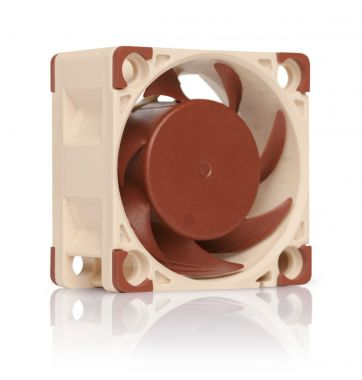
\includegraphics[width=6cm]{./pic/noctua-1.jpg}
    \end{subfigure}
    \begin{subfigure}{0.4\textwidth}
        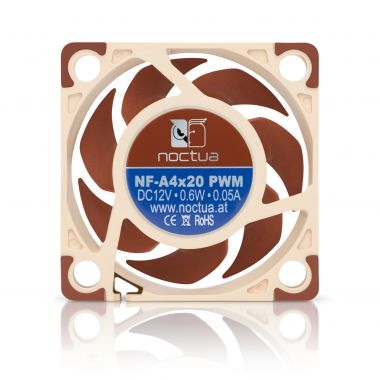
\includegraphics[width=6cm]{./pic/noctua-2.jpg}
    \end{subfigure}
    \caption{Der Lüfter von \textit{Noctua} \autocite{noctua-fan}.}
    \label{fig:fan-pic}
\end{figure}

\begin{table}[p]
    \centering
    \begin{tabular}{|l|l|l|l|}
        \hline
        \textbf{Lüfter Pin} & \textbf{Farbe} & \textbf{Funktion}  & \textbf{Anschluss} \\
        \hline
        \hline
        1 & \textcolor{black}{$\blacksquare$ Schwarz} & \gls{gnd} & \gls{gnd} \\
        \hline
        2 & \textcolor{Goldenrod}{$\blacksquare$ Gelb} & \gls{vcc} & $5\si{\volt}$ \\
        \hline
        3 & \textcolor{ForestGreen}{$\blacksquare$ Grün} & Tach & \gls{nc} \\
        \hline
        4 & \textcolor{blue}{$\blacksquare$ Blau} & \gls{pwm} & \gls{pwm} von \texttt{555} \\
        \hline
    \end{tabular}
    \caption{\gls{pwm} Lüfter Pinout Tabelle}
    \label{tab:fan-pinout}
\end{table}
